% !TeX root = Bericht.tex
% !TeX spellcheck = en_US
\section{Theory}
\label{sec:theorie}
This section describes all relevant formulas needed to understand the experiment. The theory refers to the script \cite{eom}. 
\subsection{Pockels- and Kerr-effect}
An electro-magnetic wave, which passes non-magnetic, dielectric material, causes charges to oscillate. This behaviour changes optical properties like the refractive index $n$. The exact behaviour is complicated, but since the $n$ changes little with respect to $E$, we can expand it into a Taylor series of the form
\begin{equation}
	n(E)=n_0 - \frac{1}{2}rn_0^3E - \frac{1}{2}sn_0^3E^2 + \dots.
\end{equation}
Here, $a_1 = -rn_0^3/2$ and $a_2 = -sn_0^3$ are the series coefficients obtained via first and second order derivatives and $n_0$ represents the refractive index without external fields. Expressing the coefficients $a_1$ and $a_2$ in this way allows the electric impermeability $\eta = \epsilon_0/\epsilon = 1/n^2$ to adopt the simple form
\begin{equation}\label{eqn:eta}
	\eta(E) = \eta_0 + rE + sE^2 + \dots.
\end{equation}
Usually, the second order term is already tiny and can be neglected. Refractive index and impermeability then follow a linear trend with increasing $E$. This effect is called the Pockels-effect with the corresponding Pockels coefficient $r$. 

For materials with inversion symmetry, the first order term in the expansion has to equal zero since the polarity of $E$ does not matter. Thus, the the second order term has to be considered where refractive index is proportional to the square of the electric field. This effect, typically much lower than Pockels-effect, is called Kerr-effect. 

\subsection{Anisotropic materials}
When studying the Pockels-effect, anisotropic materials have to be used. However this means, that material properties like $n$, $\epsilon$ and $\eta$ are no longer independent of the orientation of the material. They have to be extended to $3\times3$ matrices, in a basis of our choice. We choose a basis in which $\epsilon$ is diagonal, with eigenvalues $\epsilon_i$. This basis defines three directions, also known as optical axes, in which the polarization of propagating light does not change. The axes have distinct refractive indices $n_i^2 = \epsilon_i/\epsilon_0$. Any incident light can be decomposed onto the optical axes.

Before studying the properties of anisotropic materials, we have to generalise \autoref{eqn:eta} to comply with the extension to matrices. The new relation
\begin{equation}\label{eqn:tensoreta}
	\eta_{ij}(\vec{E}) = (\eta_0)_{ij} + \sum_k r_{ijk}E_k + \sum_{kl} s_{ijkl}E_kE_l + \dots
\end{equation}
contains a vectorial electric field $\vec{E}$ and tensorial generalisations of both Pockels ($r_{ijk}$) and Kerr ($s_{ijkl}$) coefficients. These contain $3^3$ and $3^4$ components respectively, but symmetry arguments reduce the total degrees of freedom. 

Some crystals (uniaxial crystals) have only two distinct refractive indices with $n_1 = n_2 = n_o$, the refractive index of the ordinary axis, and $n_3 = n_e$ the extraordinary refractive index. In the case of an uniaxial crystal of the trigonal 3m group (such as \ch{LiNbO3}), the pockel tensor can be reduced to a $6\times3$ matrix by mapping the first two indices $i, j$ onto one index $I$. The mapping rules are listed in \autoref{table:indices}.

\begin{center}
	\captionof{table}{The mapping rules from double index $(i, j)$ onto single index $I$ are listed for a pockels coefficient of a uniaxial trigonal 3m crystal. \vspace{0.3cm}}
	\begin{tabular}{@{\extracolsep{5mm}} 
			l
			S[table-format=1]
			S[table-format=1]
			S[table-format=1]
			S[table-format=1]
			S[table-format=1]
			S[table-format=1]
		}
		\toprule
		& \multicolumn{6}{c}{\makecell{Index pair $(i, j)$}} \\
		\cmidrule(lr){2-7}
		{}
		&   {$(1, 1)$}
		&   {$(2, 2)$}
		&   {$(3, 3)$}
		&   {$(2, 3)$ or $(3, 2)$}
		&   {$(1, 3)$ or $(3, 1)$}
		&   {$(1, 2)$ or $(2, 1)$}\\
		\midrule
		Index $I$ & 1 & 2 & 3 & 4 & 5 & 6 \\
		\bottomrule
	\end{tabular}
	\label{table:indices}
\end{center}\vspace{0.5cm}

After remapping the indices, the pockels coefficient can be displayed as

\begin{equation}\renewcommand\arraystretch{0.8}
	r_{IK} = \begin{pmatrix}
		0 & -r_{22} & r_{13} \\
		0 & r_{22} & r_{13} \\
		0 & 0 & r_{33} \\
		0 & r_{51} & 0 \\
		r_{51} & 0 & 0 \\
		-r_{22} & 0 & 0
	\end{pmatrix}.
\end{equation}

We will now consider an electric field parallel to the extraordinary axis $\vec{E} = (0, 0, E)$. In such a case, the sums in \autoref{eqn:tensoreta} can be omitted and the refractive index (or impermeability for that matter) for the ordinary and extraordinary axis decouple. We are left with the following equations
\begin{align*}
	\frac{1}{n_o^2(E)} &= \frac{1}{n_o^2} + r_{13}E \\
	\frac{1}{n_e^2(E)} &= \frac{1}{n_e^2} + r_{33}E 
\end{align*}
, which can be brought into the approximate form
\begin{align}
	n_o(E) &\approx n_o + \frac{1}{2}n_o^3r_{13}E \\
	n_e(E) &\approx n_e + \frac{1}{2}n_e^3r_{33}E.
\end{align}
Here $n_o$ and $n_e$ are refractive indices without external field, whilst when considering nonzero $E$ it is explicitly mentioned ($n_o(E)$ and $n_e(E)$). Both indices depend on different elements of the pockel matrix $r_{13}$ and $r_{33}$.

\subsection{Phase and intensity modulation}
When a light wave transverses medium, its electric field $E_\mathrm{L}$ experiences a phase shift. This phase shift depends on the length of the Pockels crystal, the vacuum wavelength of the laser, the external electric field $E$, the Pockels coefficient $r$ and die refractive index without external field $n_0$. The phase shift $\phi$ is given by
\begin{equation*}
	\phi=\frac{2\pi n_0L}{\lambda_0}-\pi\frac{rn_0^3EL}{\lambda_0}. 
\end{equation*}
The electric field is created by a applying a voltage $V$ to two parallel metal plates mounted on opposite sides of the crystal acting as a plate capacitor, separated by the crystals width $d$. Using $E=V/d$, we can define the half-wave-voltage, which is the voltage needed to induce a phase shift of $\pi$. The half-wave-voltage then is 
\begin{equation}
	V_{\pi}=\frac{d}{L}\frac{\lambda_0}{r n_0^3},  \label{volt_pi_relation}
\end{equation}
which simplifies the term for the phase shift to 
\begin{equation}
	\phi=\frac{2\pi n_0L}{\lambda_0}-\pi\frac{V}{V_{\pi}}. 
\end{equation}
If an EOM is placed in one arm of a Mach-Zehnder interferometer, the phase shift only occurs in one beam. In the output beam, the two waves interfere. When changing the phase difference by varying the voltage, constructive or destructive interference can be achieved. The transmittance $T$ is given by 
\begin{equation}
	T(V)=\mathrm{cos}^2\left(\alpha-\frac{\pi}{2}\frac{V}{V_\pi}\right). \label{transmittance}
\end{equation}
In this relation, $\alpha$ is a fixed phase. If $\alpha$=0 is reached in an experimental setup, the interferometer functions as an optical switch, by changing the input voltage from 0 to $V_\pi$. This, however, only works if 50/50 beam splitters are used. 
\subsection{Modulation of a circularly polarised laser beam}

Upon examination of a circularly polarised laser beam that is transmitted through the EOM, it becomes evident that the electric field exhibits a horizontal and vertical component, which follows the ordinary and extraordinary optical axes, respectively. In the case of circular polarisation, the intensity is distributed equally on both axes. In order to predict the $V_\pi$ for this case, it is possible to utilise the $V_{\pi,o}$ and $V_{\pi, e}$. These are the half-wave voltages for the ordinary and extraordinary optical axis. In accordance with the definition of the have wave voltage, the total phase shift must be equal to $\pi$. This implies that  
$$ \phi = \phi_0-\pi\frac{V}{V_\pi}=\phi_o+\phi_e=\phi_{0,o}-\pi\frac{V}{V_{\pi,o}}+\phi_{0,e}-\pi\frac{V}{V_{\pi,e}}$$
leading to 
$$\frac{1}{V_\pi}=\frac{1}{V_{\pi,e}}+\frac{1}{V_{\pi,e}}$$ \label{EQ:VPI}. 
This conclusion can be reached simply by comparing the coefficients of efficiency.

\subsection{Optical contrast}
Lastly, we will introduce the optical contrast, which is a measure for how well one can distinguish high from low intensities in a signal. It's formal definition
\begin{equation}\label{eqn:contrast}
	\mathrm{contrast} = \frac{I_{\mathrm{max}} - I_{\mathrm{min}}}{I_{\mathrm{max}} + I_{\mathrm{min}}} \cdot 100 \%
\end{equation}
is given by the ratio between intensity difference between maximum and minimum intensity $I_{\mathrm{max}} - I_{\mathrm{min}}$ and the summed intensity $I_{\mathrm{max}} + I_{\mathrm{min}}$.

%\begin{figure}[H]
%    \centering
%    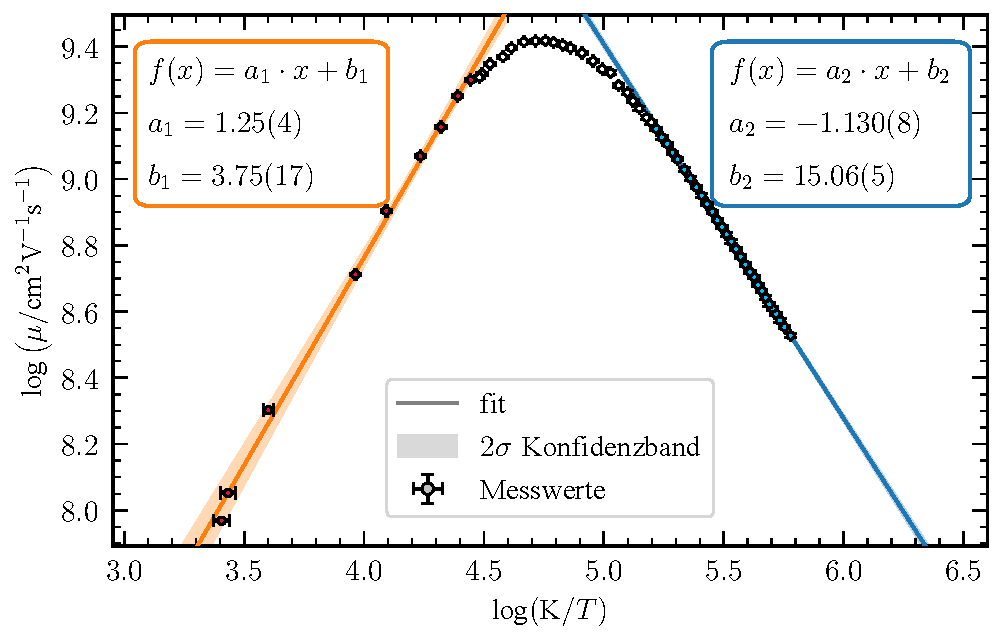
\includegraphics[width=\textwidth]{plot3.pdf}
%    \caption{}
%    \label{fig:plot3}
%\end{figure}

